%学会発表レジュメテンプレート ver. 1.1

%2段落にするためにtwocolumnを追加
\documentclass[uplatex,twocolumn]{jsarticle}
\usepackage[top=20mm,bottom=20mm,left=20mm,right=20mm]{geometry}
\usepackage[T1]{fontenc}
\usepackage{txfonts}
\usepackage{wrapfig}
\usepackage[expert,deluxe]{otf}
\usepackage[dvipdfmx,hiresbb]{graphicx}
%ハイパーリンクに色がつかないようにするため、hidelinksを追加
\usepackage[dvipdfm,hidelinks]{hyperref}
\usepackage{pxjahyper}
%2段落にするために以下を追加
\usepackage{multicol}


\makeatletter
  \renewcommand{\section}{%
    \if@slide\clearpage\fi
    \@startsection{section}{1}{\z@}%
    {\Cvs \@plus.5\Cdp \@minus.2\Cdp}% 前アキ
    {.5\Cvs \@plus.3\Cdp}% 後アキ
    %{\normalfont\Large\headfont\raggedright}}
    {\normalfont\raggedright}}

  \renewcommand{\subsection}{\@startsection{subsection}{2}{\z@}%
    {\Cvs \@plus.5\Cdp \@minus.2\Cdp}% 前アキ
    {.5\Cvs \@plus.3\Cdp}% 後アキ
    %{\normalfont\large\headfont}}
    {\normalfont}}

  \renewcommand{\subsubsection}{\@startsection{subsubsection}{3}{\z@}%
    {\Cvs \@plus.5\Cdp \@minus.2\Cdp}%
    {\z@}%
    %{\normalfont\normalsize\headfont}}
    {\normalfont}}
    
  %2段落で画像貼り付けをするために以下を追加    
  \newenvironment{figurehere}
    {\def\@captype{figure}}
    {}      
    
\makeatother
%ここから上を編集する必要はない.





\title{\vspace{-14mm}大学入試センター試験数学1・Aを用いた数式処理システムの性能評価 \footnotemark[0]}
\author{森谷 慧士 \footnotemark[2] \\ 千葉工業大学 社会システム科学部 プロジェクトマネジメント学科\footnotemark[2]}
\date{}%日付を入れる必要はない.
\pagestyle{empty}%ページ番号は振らない.
\begin{document}
%タイトルを1段落にするために以下を追加
\twocolumn[
	\maketitle
]

%脚注の追加をするために以下を追加
\begingroup
\def\thefootnote{\fnsymbol{footnote}}
\footnotetext[0]{英語の研究タイトル}
\footnotetext[2]{英語の氏名・Department of Project Management, Social System Sciences, Chiba Institute of Tchnology}
\endgroup




\section{研究の背景}

2014年11月にはみずほ銀行がコールセンターにIBMの人工知能であるWatsonを導入したことで話題となった\cite{mizuho2014}.人工知能を利用することで,膨大な解答例データの中から最適な回答案を優先的に表示させ,コールセンターの対応時間の短縮につなげることができる.このように,ビジネス内での様々なシステムに人工知能が導入され始めている.
 
2014年11月に「ロボットは東大に入れるか」という研究が取り上げられて話題となった\cite{tourobo2014}.これは,人工知能を利用して東大入試を突破できる計算機プログラムを開発することにより,「思考するプロセス」を研究しようというものである.この研究により,人工知能が思考して学習するというプロセスを得ることになり,SFに登場するような思考し自己学習をする人工知能を搭載したシステムやロボットが登場してくると推測される.

政府が進めているプロジェクトもある.「第4の産業革命」というロボットや,人工知能を活用した革新的なものづくりを目指す取り組みが始まった.この取り組みは,ドイツで「インダストリー4.0」と呼ばれる動きから始まり,日本政府も経済産業省を中心に取り組まれ始めている\cite{sangyou2014}.

2015年2月には,ソフトバンクが人工知能を搭載したヒト型ロボットの「Pepper」を発売した.Pepperは,感情認識と自立感情を持つロボットである.本体に搭載された各種センサーで状況を判断し,独自のアルゴリズムでロボットの機能を制御するアプリを自律的に制御する.また,カメラや音声認識技術によって人の表情と声からその人の感情を推定する感情認識機能も搭載している.これにより,Pepperは人とコミュニケーションを通じて和ませ,喜ばすことが可能となる.今後は,ネットワークと接続し,更に進化することが望まれる\cite{softbank}.





\section{研究の目的}

人工知能を使用する際に,我々がプロジェクトマネージャとして必要となる知識が存在する.

そこで本研究では,人間が問題を数学的表現に変換する際に必要となる知識を調査する.本研究では,Mathematicaを使用する.Mathematicaとは数式処理を行うツールである.今回は,数式処理を実行させるためにMathematicaに与える命令は何かを研究する.





\section{プロジェクトマネジメントとの関連}

プロジェクトを進める際に,プロジェクトメンバの一人として人工知能を導入する.また,ステークホルダーとして人工知能を導入する.これらの動作をすることで,プロジェクトマネージャを人工知能が補佐することが出来る.




\section{研究の方法}

今回は,数学の問題を解く過程を二つにする.

一つ目は,数学の問題を理解し,数学的知識を利用して計算式などの数学的表現に変換する過程である.二つ目は,数学的表現に変換した式を数式処理して,値を求める過程である.

今回は後者を人工知能に処理させ,前者を人間が処理するように分ける.その際に,人間がいかに簡潔に問題文を処理できるかを研究する.

今回は大学入試センター試験の数学をMathematicaに処理させる.そして,使用したコードの数と,利用した数学的知識を集計する.







\section{数式処理システム}

\subsubsection{Mathematicaとは}

Mathematica とは,あらゆる分野の計算に対応する豊富な関数と高度なグラフィック機能を備えた数式所為システムである.Mathematica を提供しているウルフラム・リサーチ社を創業したスティーブン・ウルフラム氏が考案し広く使われている数式処理システムである.



\subsubsection{Wolfram言語とは}

Mathematicaは,Wolfram言語を利用する.Wolfram言語とは,ウルフラム・リサーチ社が開発した,非常に汎用性の高いマルチパラダイムプログラミング言語である.

Wolfram言語は,Mathematica独自のノートブックインターフェイス上で利用することで,インタラクティブなデータ処理を行うスクリプトとして利用できる.さらに,アプリケーションの開発言語として利用すれば,GUIから高度な計算エンジンまで,一貫して一つの環境下で開発を行うことが出来る.

Wolfram言語は,汎用的なデータベースやインターネット上のデータを直接取り組むことができ,5000もの組み込み関数を内蔵しているため,わずか数行でも高度なアプリケーションも開発できる.また,Wolfram言語はMathematicaだけでなくWolfram社が無償で提供しているWolfram Alphaでも利用できる\cite{mitubisi}.





\section{成果物のイメージ}

試験の年数を重ねることで,新しく使用するコードの種類が減少し,新しくコードを増やすことがなくなると考える.

また,成果物をグラフとし,横軸に実施年数をとり,縦軸にコードや使用した数学的知識をとる.



\section{調査方法}

今回は、前述のとおり数学の問題を解く過程を二つにする.第一工程では,大学入試センター試験の数学の問題をできるだけ人間が頭を使わずに,素直に数学的表現に翻訳する.

大学入試センター試験の問題は,受験生が紙と鉛筆だけで解けるように作られているため,出来る限りMathematica が問題を処理できるように式に変換する.この際に,使用した数学的知識を集計し,統計を取る.

第二工程では,第一工程で数学的表現に翻訳した式をMathematica に与えて数式処理を行う.この工程では,Mathematica が式を最適に処理できるコードを与えて,最適解を得る.この際に,使用したコードの種類を集計し,統計を取る.

\section{調査結果}

現在までに,2009~2015年までのセンター試験の数学1・A をMathematicaに処理させた.そして,処理したコードが2年連続して新たに現れることがなくなったため,一度処理させる作業を中断し統計を取ることにした.

\begin{figure}[!htb]
\centering
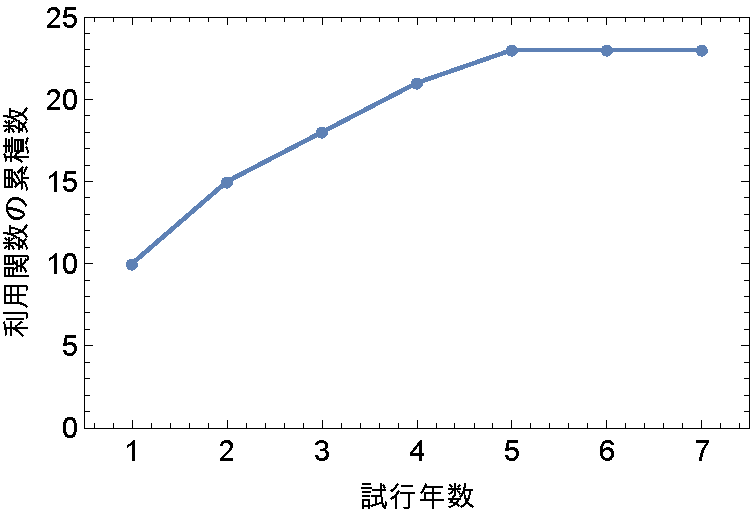
\includegraphics[width=8cm]{code.pdf}
\caption{MathematicaOnlineのホームページ}\label{サンプル図}
\end{figure}

結果,使用したコードは,SolveやSimplify等23種類となった.


\section{考察}

以下のように研究を進める計画である.

以上の結果より,人工知能であるMathematicaにセンター試験の数学1・Aを解かせる際に使用数コードは,一定の種類となることがわかる.





\bibliographystyle{junsrt}
\bibliography{biblio}%「biblio.bib」というファイルが必要.

\end{document}